\documentclass[a4paper,10pt]{article}
\usepackage{graphicx}
\usepackage{caption}
\usepackage{enumitem}
\usepackage{multicol}
\usepackage{mathtools}
\usepackage{amsmath,amsthm,amssymb,cancel,bm}
\usepackage{floatrow}
\setcounter{tocdepth}{2}
\usepackage{geometry}
\geometry{total={210mm,297mm},
left=25mm,right=25mm,%
bindingoffset=0mm, top=20mm,bottom=20mm}
\newcommand{\linia}{\rule{\linewidth}{0.5pt}}
\AtBeginDocument{%
   \setlength\abovedisplayskip{-3pt}
   \setlength\belowdisplayskip{5pt}}

\usepackage{hyperref}
\hypersetup{colorlinks=true,linkcolor=blue,citecolor=green,filecolor=cyan,urlcolor=magenta}

% my own titles
\makeatletter
\renewcommand{\maketitle}{
\begin{center}
\vspace{2ex}
{\huge \textsc{\@title}}
\vspace{1ex}
\\
\linia\\
\@author
\vspace{4ex}
\end{center}
}
\makeatother

% custom footers and headers
\usepackage{fancyhdr,lastpage}
\pagestyle{fancy}
\lhead{}
\chead{}
\rhead{}
\renewcommand{\headrulewidth}{0pt}
\lfoot{General Qualifying Exam Solutions}
\cfoot{}
\rfoot{Page \thepage\ /\ \pageref*{LastPage}}

% --------------------------------------------------------------
%
%                           TITLE PAGE
%
% --------------------------------------------------------------

\begin{document}
\hfill{\textit{Last modified \today}}
\title{General Qualifying Exam Solutions: Physics}
\author{Jessica Campbell, Dunlap Institute for Astronomy \& Astrophysics (UofT)}
\date{\today}
\maketitle

\tableofcontents



% --------------------------------------------------------------
%
%
%                              PHYSICS 
%
%
% --------------------------------------------------------------

\newpage
\section{Physics}

% --------------------------------------------------------------
%               1. 
% --------------------------------------------------------------

\subsection{Question 1}

Draw the geometry of gravitational microlensing of one star by another, and estimate the angular displacement of the background star's image.

\subsubsection{Short answer}

Answer.

\subsubsection{Additional context}

Additional context.

\subsubsection{Follow-up Questions}

\begin{itemize}
    \item Can you derive $\phi$ from a Newtonian approach?
    \item Why/how does gravitational lensing magnify a star?
\end{itemize}

% --------------------------------------------------------------
%               2. 
% --------------------------------------------------------------

\newpage
\subsection{Question 2}

A two-element interferometer consists of two telescopes whose light is combined and interfered. Sketch the response of such an interferometer to a nearby red giant star, as a function
of the (projected) separation between the two telescopes. The red giant subtends one-fiftieth of an arc second on the sky, and the telescope operates at a wavelength of 2 microns.

\subsubsection{Short answer}

Answer.

\subsubsection{Additional context}

Additional context.

\subsubsection{Follow-up Questions}

\begin{itemize}
    \item What do the minima in the response function tell you?
\end{itemize}

% --------------------------------------------------------------
%               3. 
% --------------------------------------------------------------

\newpage
\subsection{Question 3}

What's the minimum mass of a black hole you could survive a fall through the event horizon without being ripped to shreds? Why would you be ripped to shreds for smaller black holes? How does this relate to the BH mass range for which we expect tidal disruption flares caused by shredding main-sequence stars?

\subsubsection{Short answer}

Answer.

\subsubsection{Additional context}

Additional context.

\subsubsection{Follow-up Questions}

\begin{itemize}
    \item How would you estimate the maximum tidal acceleration a star can withstand?
    \item Why is it enough to know if the surface of the star will be disrupted?
\end{itemize}

% --------------------------------------------------------------
%               4. 
% --------------------------------------------------------------

\newpage
\subsection{Question 4}

How is synchrotron radiation generated, and how was it used to demonstrate the energy required to power radio galaxies?

\subsubsection{Short answer}

Answer.

\subsubsection{Additional context}

Synchrotron radiation from the Galaxy was the first emission detected in radio astronomy, although it was not until the 1950s when detailed radio maps of the Galaxy were produced, that the connection was made between radio emission and the synchrotron mechanism. Synchrotron radiation, also known as \textbf{magnetobremsstrahlung radiation}, is a type of \textbf{non-thermal radiation} emitted by relativistic electrons being deflected by the magnetic field of the ISM. It occurs in the diffuse ISM and in SN remnants, due in part to electron acceleration associated with the supernova blastwave and in part to increased magnetic field strengths in the shocked gas. This radiation dominates the sky brightness at frequencies $\nu\lesssim1\,{\rm GHz}$. Figure \ref{fig:haslam408} shows the all-sky radio map at $408\,{\rm MHz}$.

\begin{figure}[h]
    \centering
    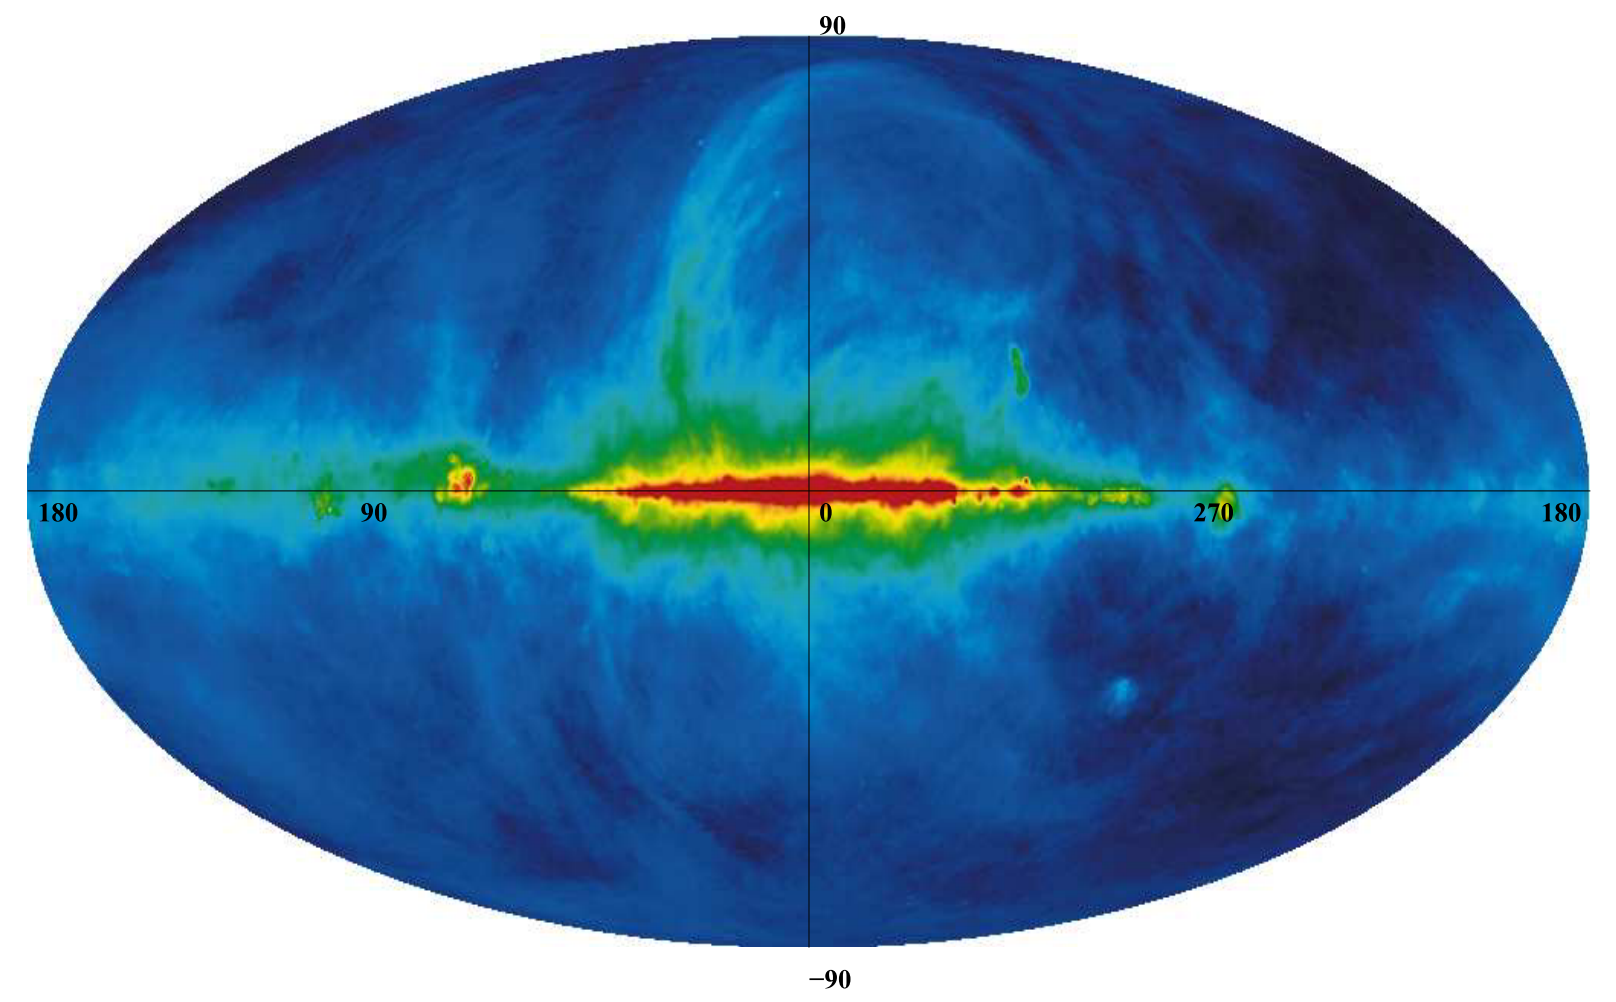
\includegraphics[width=12cm]{figures/Haslam408.png}
    \caption{\footnotesize{The synchrotron emission at $408\,{\rm MHz}$ across the entire sky in Galactic coordinates. As expected the emission is concentrated along the Galactic plane. The noticeable feature known as Loop I is clearly arching up from $\ell=55^\circ$ towards the North Galactic Pole. This figure is adapted from Haslam et al. (1981). Figure taken from Newton-McGee (2009).}}
    \label{fig:haslam408}
\end{figure}

{\noindent}\textbf{Cosmic rays} (i.e., high energy nuclei and electrons) are an important component of the ISM along with magnetic fields and interstellar gas. While the origin of cosmic rays is still not comprehensively understood, it is believed that the electrons with an energy approaching $100-1000\,{\rm TeV}$ have been accelerated in SNRs, suggesting this is one mechanism for the primary formation of cosmic rays.

{\noindent}Magnetic fields accelerate these charged particles via the \textbf{Lorentz force}. The acceleration is given by

\begin{align*}
    \frac{{\rm d}}{{\rm d}\tau}(m\gamma v) = q\left(\frac{\vec{v}}{c}\times\vec{B}\right) ~ [{\rm N}]
\end{align*}

{\noindent}where $m$ is the mass of the particle with charge $q$, $\tau$ is the retarded time, the Lorentz factor  $\gamma=(1 v^2/c^2)^{-1/2}$, and $\vec{B}$ is the magnetic field. The trajectory of the particle is \textit{helical}, with a \textbf{gyration frequency} $\omega_B$ and \textbf{pitch angle} $\theta$ (where $\theta=90^\circ$ for a circular orbit, and $\theta=0^\circ$ for a particle trajectory parallel to $\vec{B}$).

\begin{figure}[h]
    \floatbox[{\capbeside\thisfloatsetup{capbesideposition={right,top},capbesidewidth=4cm}}]{figure}[\FBwidth]
    {\caption{\footnotesize{\\The trajectory of a relativistic electron spiraling in a magnetic field B with a pitch angle $\theta$. The electric field $E$ is polarized parallel to the orbital plane. The synchrotron emission is emitted in a highly beamed cone. This figure is adapted from Kraus (1986). Figure taken from Newton-McGee (2009).}}
    \label{fig:synchrotrondiagram}}
    {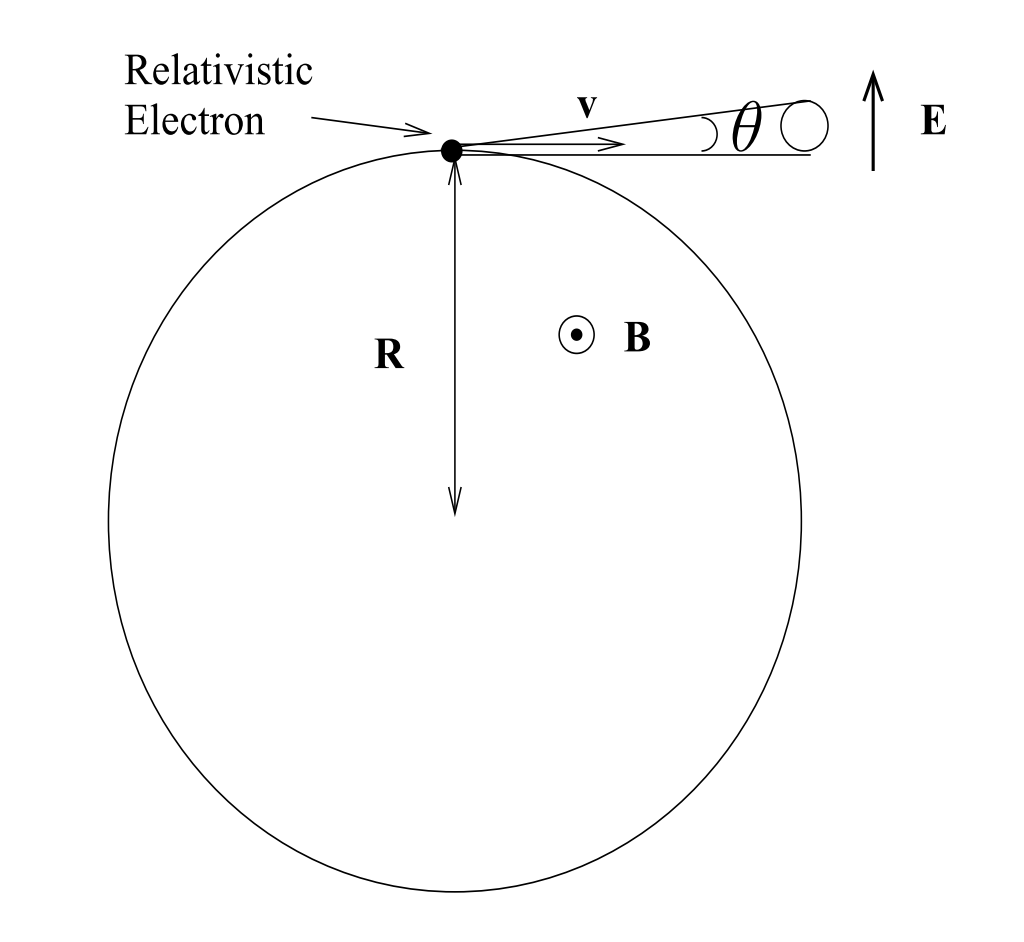
\includegraphics[width=6cm]{figures/SynchrotronDiagram.png}}
\end{figure}

{\noindent}A charged particle deflected by magnetic fields while moving at relativistic speeds emits synchrotron radiation during this acceleration. The main properties of the synchrotron radiation are the following:

\begin{itemize}
    \item high intensity;
    \item very broad and continuous spectral range from infrared up to the hard x-ray region;
    \item natural narrow angular collimation;
    \item high degree of polarization;
    \item pulsed time structure.
\end{itemize}

The graphical representation of synchrotron radiation, depicted in Figure \ref{fig:synchrotrondiagram}, shows that the velocity vector of the particle generates the surface of a cone, with the synchrotron emission beamed within the surface of the cone, at an angle of:

\begin{align*}
    \theta = \pm \frac{mc^2}{E} ~ [{\rm rad}].
\end{align*}

{\noindent}On the surface of the cone the radiation is $100\%$ linearly polarized with its electric field in the direction $-\vec{v}\times\vec{B}$, where $v$ is the direction of propagation of the electron. The degree of linear polarization, called the polarization fraction $p$, is independent of frequency and depends on the spectral index of the cosmic ray electrons:

\begin{align*}
    p(\alpha) = \frac{3-3\alpha}{5-3\alpha} ~ [{\rm dimensionless}].
\end{align*}

{\noindent}In order to understand the angular and spectral distribution of the emitted radiation of synchrotron radiation, let us remind ourselves of the emission from a classical electron moving at a speed $v$ much lower than the speed of light ($v\ll c$). In this case the emitted pattern is similar to that of an oscillating dipole with its maximum of intensity in the direction perpendicular to the acceleration and does not depend on the electron speed. For a relativistic effect, when the speed of the emitting electrons increases to relativistic values ($v\approx c$) the radiation pattern is compressed into a narrow cone in the direction of motion, resulting into an emission tangential to the particle orbit. The vertical half-opening angle $\theta$ is given by

\begin{align*}
    \theta \approx \frac{mc^2}{E} \approx \frac{1}{\gamma} ~ [{\rm rad}].
\end{align*}

{\noindent}See Figure \ref{fig:synchrotronorbits}.

\begin{figure}[h]
    \centering
    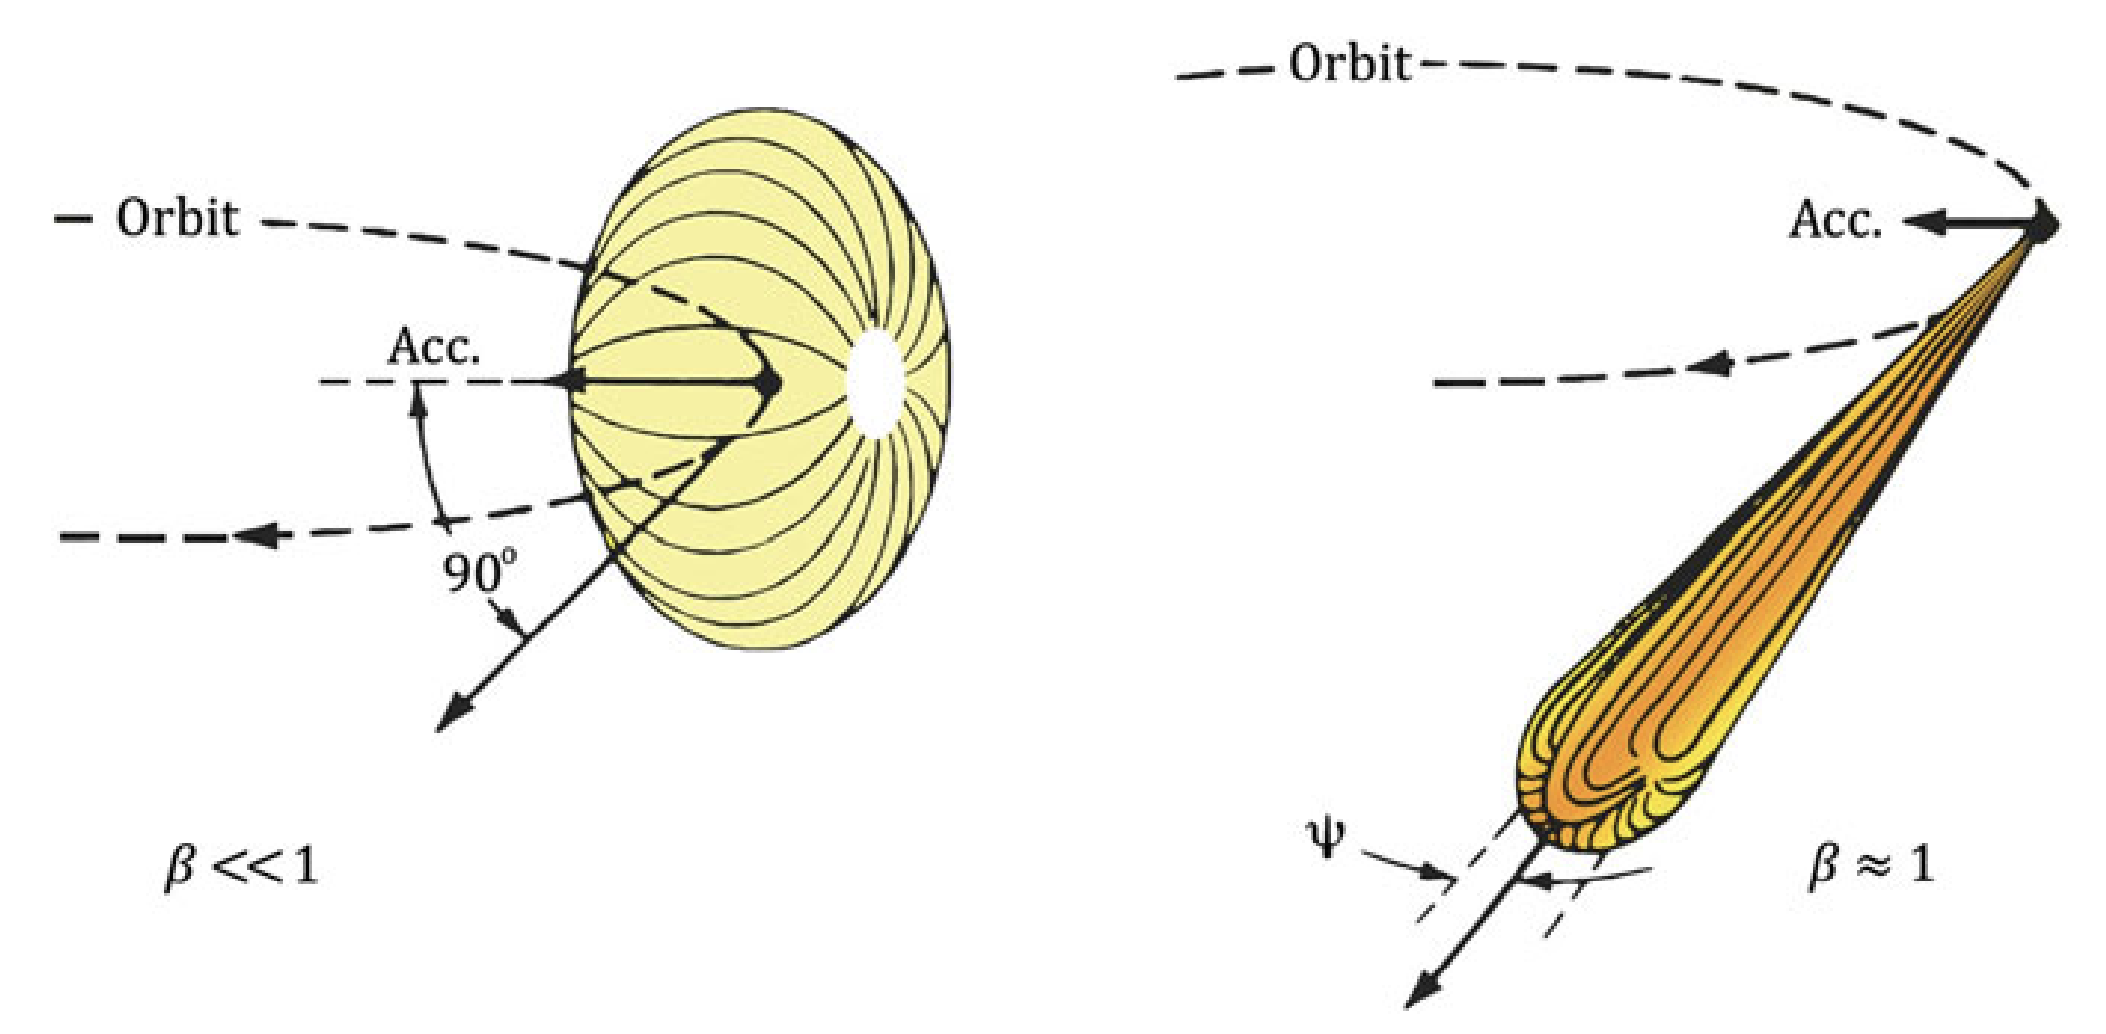
\includegraphics[width=12cm]{figures/SynchrotronOrbits.png}
    \caption{\footnotesize{Qualitative radiation patterns related to charged particles moving in a circular orbit. The dipole pattern is achieved for slow particles when $v/c\ll1$ (left); this is distorted into a narrow cone when $v/c\approx1$ (right). Figure taken from Mobilio et al. (2015).}}
    \label{fig:synchrotronorbits}
\end{figure}

{\noindent}The radiated power from the accelerating charge is given (in cgs units) by

\begin{align*}
    P = \frac{2}{3}\frac{q^4}{m^2c^5} (\gamma\nu)^2 (B\sin\theta)^2 = 2.37\times10^{-15} \left(\frac{E}{{\rm erg}}\right)^2 \left(\frac{B\sin\theta}{\mu{\rm G}}\right)^2 ~ [{\rm erg\,s^{-1}}]
\end{align*}

{\noindent}where the final equality is given for electrons in particular, since the dependence on the mass-to-charge ratio means that electrons are by several orders of magnitude dominant over protons or ions in generating synchrotron radiation. The synchrotron power peaks at the \textbf{characteristic frequency} (in Hz) of

\begin{align*}
    \nu_c = \frac{3}{4\pi}\frac{q}{mc}\gamma^2(B\sin\theta) = 6.26\times10^3 \left(\frac{E}{{\rm erg}}\right)^2 \left(\frac{B\sin\theta}{\mu{\rm G}}\right) ~ [{\rm Hz}].
\end{align*}

{\noindent}This equation tells us that for radio observations (frequencies at or above tens of ${\rm MHz}$) and with typical magnetic field strengths of order $\mu{\rm G}$, the observed population of electrons have $\gamma\gg1$. The radiation is thus highly beamed (width $\sim\gamma^{-1}$) in the direction of the velocity vector. The population of electrons has a power-law energy distribution given by

\begin{align*}
    n(\gamma){\rm d}\gamma = n_0\gamma^{-p}{\rm d}\gamma ~ [{\rm eV^{-1}}]
\end{align*}

{\noindent}where a typical value for the power law index is $p\approx2.5$. The resulting synchrotron luminosity is thus also a power law,

\begin{align*}
    L_\nu \propto \nu^{-(p-1)/2}\equiv \nu^{-\alpha} ~ [{\rm erg\,s^{-1}}]
\end{align*}

{\noindent}with a typical spectral index $\alpha=0.75$ for $p=2.5$. The particles lose energy due to the power emitted with a characteristic timescale of

\begin{align*}
    \tau_{\rm syn} = \frac{\gamma}{{\rm d}\gamma/{\rm d}\tau} = 4\pi\frac{mc}{\sigma_T}\gamma^{-1}(B\sin\theta)^{-2} ~ [{\rm yr}]
\end{align*}

{\noindent}where the \textbf{Thomson cross-section} $\sigma_T=8\pi q^4/3m^2c^4$. Since $\tau_{\rm syn}$ is shorter for more energetic electrons (higher $\gamma$) the power law in the number density $n(\gamma){\rm d}\gamma$ steepens with time (often corresponding to distance from the site of cosmic ray acceleration), therefore increasing the value of $\alpha$. This is referred to as \textbf{synchrotron aging}. Substituting for the characteristic synchrotron frequency $\nu_c$, we can see that

\begin{align*}
    \left(\frac{\tau_{\rm syn}}{{\rm yr}}\right) = 1.06\times10^9 \left(\frac{B\sin\theta}{\mu{\rm G}}\right)^{-1.5} \left(\frac{\nu_c}{{\rm GHz}}\right)^{-0.5}.
\end{align*}

{\noindent}The spectrum of synchrotron radiation must be related to the detailed variation of the electric field as seen by an observer. Because of beaming effects the emitted radiation fields appear to be concentrated in a narrow set of directions about the particle's velocity. The observer will see a pulse of radiation confined to a time interval much smaller than the gyration period. The spectrum will thus be spread over a much broader region than one of order $\omega_B/2\pi$. This is an essential feature of synchrotron radiation.

{\noindent}Non-thermal cosmic radio emission was first thought to originate in stellar atmospheres (the \textbf{radio star hypothesis}). This hypothesis seemed quite reasonable at first glance in view of the existence of quite intense sporadic radio emission from the Sun. It is easy to see, however, that to explain the observed data, these hypothetical radio stars would need to possess extremely unusual properties. The discovery of a quasi-spherical component of the general galactic radio emission imposed severe demands on the radio star hypothesis. For instance, it became clear in this connection that sources of non-thermal galactic radio emission were distributed principally in the galactic halo, the discovery of which had been made only a short time before. Nevertheless, the radio star hypothesis was still not abandoned. If, on the other hand, we equate the general galactic radio emission with synchrotron radiation we then obtain completely probable and useful estimates of the intensity of interstellar fields and the concentration of relativistic electrons. Such estimates are also encouraging in the case of discrete sources. The radio star hypothesis was thus abandoned as early as the beginning of 1953 and the synchrotron character of the major part of non-thermal cosmic radio emission was accepted. 

% --------------------------------------------------------------
%               5. 
% --------------------------------------------------------------

\newpage
\subsection{Question 5}

What are ``forbidden lines'' of atomic spectra? In what conditions are they observationally important? In what conditions do they control the temperature of interstellar material?

\subsubsection{Short answer}

Answer.

\subsubsection{Additional context}

Additional context.

\subsubsection{Follow-up Questions}

\begin{itemize}
    \item What are some common examples of forbidden lines?
    \item When do you get forbidden line absorption?
    \item What kind of radiation can be absorbed by forbidden line absorption?
    \item Can we observe any forbidden lines on Earth?
    \item What is the lifetime of the 21 cm line?
    \item At what redshifts do CMB photons get absorbed by 21 cm transitions?
    \item At what redshifts do you get neutral hydrogen?
    \item How would you estimate the lifetime from the maximum density where the line isn't washed out?
    \item Collisions happen much more frequently; why is the 21 cm line still visible?
    \item Why does forbidden line emission cool the gas?
    \item Why are they \textit{so good} at cooling the gas?
\end{itemize}

% --------------------------------------------------------------
%               6. 
% --------------------------------------------------------------

\newpage
\subsection{Question 6}

What is a polytropic equation of state? Give examples of objects for which this is a very good approximation, and explain why it is.

\subsubsection{Short answer}

Answer.

\subsubsection{Additional context}

Additional context.

% --------------------------------------------------------------
%               7. 
% --------------------------------------------------------------

\newpage
\subsection{Question 7}

What was the solar neutrino problem, and how was it resolved?

\subsubsection{Short answer}

Answer.

\subsubsection{Additional context}

Additional context.

\subsubsection{Follow-up Questions}

\begin{itemize}
    \item Can neutrinos account for all of the dark matter in the Universe?
    \item If there was a fourth neutrino flavour, how would we detect it?
    \item Why is the first step of the p-p chain not where we looked for neutrino signatures? (i.e., not energetic enough)
\end{itemize}

% --------------------------------------------------------------
%               8. 
% --------------------------------------------------------------

\newpage
\subsection{Question 8}

Why is nuclear fusion stable inside a main-sequence star? Under what conditions is nuclear fusion unstable? Give examples of actual objects.

\subsubsection{Short answer}

Answer.

\subsubsection{Additional context}

Additional context.

\subsubsection{Follow-up Questions}

\begin{itemize}
    \item Can main sequence stars have unstable nuclear fusion?
    \item If I suddenly increase the core temperature of a star by 20\%, how quickly does the star respond?
    \item What happens when you ignite fusion in a white dwarf? Explain using explicit thermodynamics what happens when you turn up the temperature or reaction rate in the core of the star (i.e. explain adiabatic expansion and contraction).
\end{itemize}

% --------------------------------------------------------------
%               9. 
% --------------------------------------------------------------

\newpage
\subsection{Question 9}

Why do neutrons inside a neutron star not decay into protons and electrons?

\subsubsection{Short answer}

Answer.

\subsubsection{Additional context}

Additional context.

\subsubsection{Follow-up Questions}

\begin{itemize}
    \item What sort of products come from NS-NS mergers?
    \item What are typical photon energies emitted from each of these scenarios?
\end{itemize}

% --------------------------------------------------------------
%               10. 
% --------------------------------------------------------------

\newpage
\subsection{Question 10}

What is the typical temperature of matter accreting on a star, a white dwarf, a neutron star, a stellar mass black hole, and a supermassive black hole? In what wavelength range would one best find examples of such sources?

\subsubsection{Short answer}

Answer.

\subsubsection{Additional context}

Additional context.

\subsubsection{Follow-up Questions}

\begin{itemize}
    \item How does the accretion process work?
    \item If you don't assume a blackbody, and just dump a bunch of material onto a star and it can't radiate away, what is the maximum temperature it can reach?
\end{itemize}

% --------------------------------------------------------------
%               11. 
% --------------------------------------------------------------

\newpage
\subsection{Question 11}

You don't usually need to cool down the detectors for short wavelength (e.g., X-ray) observations, but it's critical to cool down the detectors in long wavelength (e.g., far-IR) observations. Why is this, and why is it not necessary for radio observations?

\subsubsection{Short answer}

Answer.

\subsubsection{Additional context}

Additional context.
% --------------------------------------------------------------
%               12. 
% --------------------------------------------------------------

\newpage
\subsection{Question 12}

Compare the S/N ratios between the following two cases where photon noise is dominant (assume an unresolved point source): [A] 1-minute exposure with a 10-m telescope; [B] 10-minute exposure with a 1-m telescope.

\subsubsection{Short answer}

Answer.

\subsubsection{Additional context}

Additional context.

% --------------------------------------------------------------
%               13. 
% --------------------------------------------------------------

\newpage
\subsection{Question 13}

Describe linear and circular polarizations of electromagnetic waves and give examples of their relevance to astronomical observations.

\subsubsection{Short answer}

Answer.

\subsubsection{Additional context}

Additional context.

% --------------------------------------------------------------
%               14. 
% --------------------------------------------------------------

\newpage
\subsection{Question 14}

What's the field of view of a $2{\rm K}\,\times\,2{\rm K}$ CCD camera on a $5\,{\rm m}$ telescope with $f/16$ focal ratio? The pixel size of the CCD is $20\,\mu$m. Now, let’s bring this to a $10\,{\rm m}$ telescope with the same focal ratio. Explain how the field of view changes on the $10\,{\rm m}$ telescope (compared to that of the $5\,{\rm m}$ telescope) based on the Etendue conservation rule.

\subsubsection{Short answer}

Answer.

\subsubsection{Additional context}

Additional context.

\subsubsection{Follow-up Questions}

\begin{itemize}
    \item If you wanted a smaller FOV with the same size telescope, what would you change?
\end{itemize}

% --------------------------------------------------------------
%               15. 
% --------------------------------------------------------------

\newpage
\subsection{Question 15}

Sketch and give the equations for each of the following distributions: 1. Gaussian (Normal distribution); 2. Poisson distribution; 3. Log-normal distribution. Give two examples from astrophysics where each of these distributions apply.

\subsubsection{Short answer}

Answer.

\subsubsection{Additional context}

Additional context.

\subsubsection{Follow-up Questions}

\begin{itemize}
    \item What sort of noise do you expect for these?
    \item What extra sources of noise can you get from a CCD?
    \item Where does the noise come from, and what does the variance/standard deviation actually tell you?
    \item What property of the Gaussian distribution makes it particularly useful? (i.e., Central limit theorem.)
    \item How do we get a log-normal distribution?
    \item Why do we quote n-sigma probabilities and confidence levels with a Gaussian assumption when the actual probability distribution might not be Gaussian?
    \item If I'm doing a cosmological survey and I say I assume a Poisson distribution for radio galaxy sources and a Gaussian distribution for dust sources, why would I use two different distributions?
\end{itemize}

% --------------------------------------------------------------
%               16. 
% --------------------------------------------------------------

\newpage
\subsection{Question 16}

You are trying to determine a flux from a CCD image using aperture photometry, measuring source(+sky) within a 5-pixel radius, and sky within a 20-25 pixel annulus. Assume you find 10000 electrons inside the aperture and 8100 electrons in the sky region, and that the flux calibration is good to 1\%. What is the fractional precision of your measurement? (Ignore read noise.) More generally, describe how you propagate uncertainties, what assumptions you implicitly make, and how you might estimate errors if these assumptions do not hold.

\subsubsection{Short answer}

Answer.

\subsubsection{Additional context}

Additional context.

% --------------------------------------------------------------
%               17. 
% --------------------------------------------------------------

\newpage
\subsection{Question 17}

Suppose you measure the brightness of a star ten times (in a regime where source- noise dominates. (1) How do you calculate the mean, median, and mode and standard deviation? (2) How can you tell if any points are outliers? Say some points are outliers, what do you do now (i.e., how does this impact the calculation of the quantities in part 1)?

\subsubsection{Short answer}

Answer.

\subsubsection{Additional context}

Additional context.

\subsubsection{Follow-up Questions}

\begin{itemize}
    \item How would you go about fitting a model to your data? (i.e., Bayesian approach.)
    \item Why is using a gaussian generally a good choice?
\end{itemize}

% --------------------------------------------------------------
%               18. 
% --------------------------------------------------------------

\newpage
\subsection{Question 18}

Suppose you do an imaging search for binaries for a sample of 50 stars, and that you find companions in 20 cases. What binary fraction do you infer? Suppose a binary- star fraction of 50\% had been found previously for another sample (which was much larger, so you can ignore its uncertainty). Determine the likelihood that your result is consistent with that fraction.

\subsubsection{Short answer}

Answer.

\subsubsection{Additional context}

Additional context.

% --------------------------------------------------------------
%               19. 
% --------------------------------------------------------------

\newpage
\subsection{Question 19}

What are the primary wavelength bands at which searches for gravitational waves are conducted? What techniques are used to search in each band? What are the sources of gravitational waves in each band? What can we learn from detections (or non-detections)?

\subsubsection{Short answer}

Answer.

\subsubsection{Additional context}

Additional context.

% --------------------------------------------------------------
%               20. 
% --------------------------------------------------------------

\newpage
\subsection{Question 20}

Self-similarity is a useful idealization of many astrophysical systems. Explain what self- similarity means, when it works, and why it is so useful, and provide two examples from any field.

\subsubsection{Short answer}

Answer.

\subsubsection{Additional context}

Additional context.

% --------------------------------------------------------------
%               21. 
% --------------------------------------------------------------

\newpage
\subsection{Question 21}

Explain why diffraction-limited detectors tend to have sidelobes, and how sidelobes can be suppressed in optical and radio observations.

\subsubsection{Short answer}

Answer.

\subsubsection{Additional context}

Additional context.

% --------------------------------------------------------------
%               Resources 
% --------------------------------------------------------------

\newpage
\subsection{Resources}

\begin{itemize}
    \item Astronomical Statistics, Taylor (2004)
    \item Statistical Methods for Astronomical Data Analysis, Chattopadhyay \& Chattopadhyay (2014)
    \item Data Reduction and Error Analysis for the Physical Sciences, Bevington \& Robinson (2003)
    \item Bayesian Logical Data Analysis for the Physical Sciences, Gregory (2005)
    \item Magnetic Fields in Diffuse Media, Lazarian (2015)
    \item Optics, Hecht (2002)
    \item Astronomical Optics, Schroeder (1987)
    \item Handbook of CCD Astronomy, Howell (2006)
    \item Gravitational Waves, Thorne (1994)
    \item Gravitational Bending of Light, Edwards (2007)
    \item Gravitational Lensing, Abdo
    \item Principles of Interferometry, Jackson (2008)
    \item Astrophysics of the Interstellar Medium; Maciel (2013)
    \item Radio Polarimetry as a Probe of Interstellar Magnetism; Newton-McGee (2009)
    \item Synchrotron Radiation; Mobilio et al. (2015)
    \item Cosmic Magnetobremsstrahlung (Synchrotron Radiation); Ginzburg \& Syrovatskii (1965)
\end{itemize}

\end{document}
